\section{Application to Thermal Protection Systems}
In this section, the proposed PIROM approach is applied to the analysis of thermo-ablative multi-layered hypersonic TPS. The performance of the PIROM is evaluated in terms of the three corners of the ITM in Fig.~\ref{fig_itm}, based on parametric variations of boundary conditions and SRMs. The results show PIROM to be a promising candidate for the solution of the impossible trinity of modeling, achieving RPM-level computational efficiency and generalizability, while attaining high-fidelity model accuracy.

\subsection{Problem Definition}
Consider the two-dimensional TPS configuration shown in Fig.~\ref{fig_tps} with constant material properties within each layer, dimensions, and BCs listed in Table~\ref{table_tps}. Such configuration is representative of the TPS used for the initial concept 3.X vehicle in past studies~\cite{Klock2017}, and involves two main layers: an outer ablative layer, and an inner substrate layer. The top ablative layer may be composed of different materials, such as PICA or Avcoat, while the substrate layer is typically made of a high-temperature resistant material, such as carbon-carbon composite~\cite{Gasch2024}. The ablative layer, composed of $\tN=3$ ablative components, is subjected to strong time-varying and non-uniform heating, while the substrate layer, composed of one non-ablative component, is insulated adiabatically at the outer surface; the total number of components is thus $N=4$. 

The lumped-mass representation of the TPS configuration is shown in Fig.~\ref{fig_lumped_mass_representation}, where each component $\Omega_i$ is represented by a lumped mass with uniform temperature $\bar{u}_i(t)$. Details regarding the derivation of the LCM for this configuration are provided in Appendix~\ref{appendix_mathematical_details}. The sources of non-linearities studied in this problem originate from the coupling between the thermodynamics and temperature-dependent mesh motion, i.e., geometry-dependent matrices and temperature advection, as well as the heterogeneities across material layers. As shown in Fig.~\ref{fig_tps}, perfect thermocouple devices are placed at the surfaces of the ablative layers for the collection of the high-fidelity temperature signals that are used in the following sections for training and testing the PIROM.

\begin{figure}[htp]
    \centering
    \subfigure[\label{fig_mesh}Mesh and Geometry]{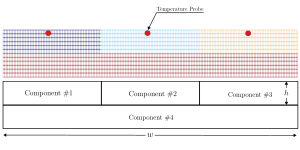
\includegraphics[width=0.9\textwidth]{./figs/mesh.png}}
    \subfigure[\label{fig_lumped_mass_representation}Lumped Mass Representation]{\includegraphics[width=0.9\textwidth]{./figs/lumped_mass_representation.png}}
    \bigskip
    \caption{Four-component TPS geometry and lumped-mass representation for the TPS.}
    \label{fig_tps}
\end{figure}

\begin{table}
    \resizebox{\textwidth}{!}{
    \begin{tabular}{ccccccc}
        \hline
        \hline
        Component & $w$ (cm) & $h$ (cm) & $\rho$ (kg/m³) & $c_p$ (J/kg·K) & $k$ (W/m·K) & $\alpha\times 10^{-6}$ (m/s·K) \\
        \hline
        \#1 & 0.3 & 0.03 & 160 & 1200 & 0.2 & 1 \\
        \#2 & 0.3 & 0.03 & 1800 & 900 & 5 & 1 \\
        \#3 & 0.3 & 0.03 & 300 & 1500 & 0.15 & 1 \\
        \#4 & 0.9 & 0.03 & 1600 & 800 & 10 & 0 \\
        \hline
        \hline
    \end{tabular}}
    \caption{Description of TPS components, including thickness $h$, density $\rho$, specific heat capacity $c_p$, thermal conductivity $k$, and SRM parameter $\alpha$.}
    \label{table_tps}
\end{table}

\subsection{Problem Parametrization}
The operating conditions of the TPS are specified by the boundary conditions, i.e., the heat flux, and the SRM matrix $\vXi$. Specifically, the heat flux on the Neumann BC is parametrized using $\xibc=\left\{\xi_1,\xi_2,\xi_3\right\}$, while the SRM is parametrized using $\xisrm=\{\alpha_1,\alpha_2,\alpha_3\}$. Thus, the heat flux and SRM over the $i$-th ablative component are expressed as,
\begin{equation}
    q_i(x,t;\xibc) = \xi_1e^{\xi_2 x}e^{\xi_3 t},\:\forall x\in\Gamma_{i,q},\quad \dot{w}_i(z_{u,i};\xisrm) = \alpha_i\left(z_{u,i} - u_{0,i}\right),\:i=1,\dots,\tilde{N}
\end{equation}
where $\Gamma_{i,q}$, $z_{u,i}$, and $u_{0,i}$ correspond to the Neumann BC surface, the surface temperature prediction, and the initial temperature of the $i$-th ablative component, respectively. The parameters $\xi_1$, $\xi_2$, and $\xi_3$ control the heat flux magnitude, spatial variation, and temporal variation, respectively. The constant $\alpha_i$ is a small material-dependent constant determined from the B' table~\cite{Padovan2024}, specifying the surface recession velocity for a given temperature.

\subsection{Data Generation}
Full-order solutions of the TPS are computed using the FEM multi-mechanics module from the \texttt{Aria} package with the mesh shown in Fig.~\ref{fig_mesh}~\cite{Clausen2024}. The mesh consists of 2196 total elements, with 366 elements for each ablative component and 1098 elements for the substrate component. Given an operating condition $\vxi=\left[\xibc,\xisrm\right]^\top$, a high-fidelity solution is computed for one minute, starting from an uniform initial temperature of $T(x,t_0)=300$ K. Each solution consist of a collection of space-time-varying temperature and displacement fields $\left\{\left(t_k,\vu^{(l)}_{\text{HF}}(t_k),\vd^{(l)}_{\text{HF}}(t_k),\vxi^{(l)}\right)\right\}_{k=0}^{p-1}$, where $p$ is the number of time steps with a step size of $\Delta t \approx 10^{-3}$. The observable trajectories are representative of near-wall thermocouple sensing of hypersonic flows involving heat transfer. At each time instance $t_k$, a temperature reading is recorded from each ablative component using the thermocouples shown in Fig.~\ref{fig_tps}, resulting in three temperature signals, i.e., the observables $\vz_{\text{HF}}\in\mathbb{R}^3$. Therefore, each full-order solution produces one trajectory of observables $\left\{\left(t_k,\vz^{(l)}_{\text{HF}}(t_k),\vxi^{(l)}\right)\right\}_{k=0}^{p-1}$. The goal of the PIROM is to predict the surface temperature and displacement as accurately as possible.

\subsubsection{Definition of Training and Testing Datasets}
The range of parameters used to generate the training $\cD_1$ and testing $\left\{\cD_2,\cD_3\right\}$ datasets are listed in Table~\ref{table_parameters}. The training and testing datasets are designed, respectively, to: (1) minimize the information that the PIROM can ``see'', and (2) to maximize the variability of test operating conditions to examine the PIROM's generalization performance. A total of $110$ normally-distributed data points for the BC parametrization are visualized in Fig.~\ref{fig_parameters}, and the corresponding observable trajectories are shown in Figs.~\ref{fig_temperature_observables} and~\ref{fig_displacement_observables}. The training dataset $\cD_1$ includes $10$ trajectories with randomly selected BC parameters from the $110$ points, with nominal SRM parameters $\xisrm = \{1, 1, 1\}\times 10^{-6}$. Note that although Fig.~\ref{fig_displacement_observables} shows the surface displacements for all ablative components in $\cD_1$, only the \textit{surface temperature is used for training the PIROM}.

\begin{table}
    \centering
    \resizebox{\textwidth}{!}{
    \begin{tabular}{ccccccc}
         & \multicolumn{6}{c}{Parameters} \\
        \hline
        \hline
        Dataset & $\xi_1\times 10^3$ & $\xi_2\times10^{-1}$ & $\xi_3\times 10^{-2}$ & $\alpha_1\times 10^{-6}$ & $\alpha_2\times 10^{-6}$ & $\alpha_3\times 10^{-6}$ \\
        \hline
        $\cD_1$ & $\left[-6.059,-5.902\right]$ & $\left[-3.501,3.152\right]$ & $\left[9.670,10.464\right]$ & $1$ & $1$ & $1$ \\
        $\cD_2$ & $\left[-6.122,-5.887\right]$ & $\left[-3.601,-3.074\right]$ & $\left[9.218,11.246\right]$ & $1$ & $1$ & $1$ \\
        $\cD_3$ & $6$ & $-3.333$ & $10$ & $\left[0.6,1.5\right]$ & $\left[0.6,1.5\right]$ & $\left[0.6,1.5\right]$ \\
        \hline
        \hline 
    \end{tabular}}
    \caption{Range of parameters $[\min,\max]$ in training and testing datasets.}\label{table_parameters}
\end{table}

Two additional datasets are generated for testing. The dataset $\cD_2$ includes the remaining $100$ BC parameter values not considered in $\cD_1$, and the high-fidelity simulation are generated with the same nominal SRM parameters. The cases in the $\cD_3$ fixes the boundary condition as shown in Fig.~\ref{fig_parameters} and varies the SRM parameters as shown in Table.~\ref{table_parameters}. The testing datasets $\cD_2$ and $\cD_3$ are \textit{out-of-distribution} (OOD) datasets, and are meant for testing the generalizability of the ROMs to unseen BCs and SRMs, respectively. 

\begin{figure}
    \centering
    \subfigure[\label{fig_parameters}BC Parameters]{\includegraphics[width=0.45\textwidth]{./figs/parameters.png}}
    \subfigure[\label{fig_temperature_observables}Surface Temperatures]{\includegraphics[width=0.45\textwidth]{./figs/temperature_observables.png}}
    \subfigure[\label{fig_displacement_observables}Surface Displacements]{\includegraphics[width=0.45\textwidth]{./figs/displacement_observables.png}}
    \caption{Boundary condition parameters, temperature observables, and displacement observables for the training and testing datasets. The variables $z_{u,i}$ and $z_{w,i}$ correspond to the surface temperature and displacement of the $i$-th ablative component, respectively.}
    \label{fig_datasets}
\end{figure}

\subsection{Performance Metrics}
The performance metrics are defined to quantitatively assess the solution to the ITM for the TPS problem. Specifically, the \textit{accuracy} metric quantifies the prediction error of the ROMs against high-fidelity solutions. The \textit{efficiency} metric quantifies the computational speedup achieved by the ROMs compared to high-fidelity simulations. The \textit{generalizability} metric quantifies the ability of the ROMs to retain accuracy when evaluated on OOD datasets. Together, these metrics provide a comprehensive evaluation of the PIROM's performance in addressing the challenges associated with modeling complex multi-physics systems. Since the generalizability metric is inherently tied to the accuracy metric when evaluated on OOD datasets, the following sections focus on defining the accuracy and efficiency metrics.

\paragraph*{Accuracy Metric} Consider one trajectory of high-fidelity surface temperature and displacement data $\left\{\left(t_k,\vz^{(l)}_{u,\text{HF}}(t_k),\vz^{(l)}_{w,\text{HF}}(t_k)\right)\right\}_{k=0}^{p-1}$ for the $l$-th operating condition in the testing datasets $\cD_2$ or $\cD_3$. The difference $e_i^{(l)}$ for the $i$-th predicted observable, denoted as $z_{i}^{(l)}$, is computed as,
\begin{equation}
    e_i^{(l)} = \frac{1}{\Delta z_i^{(l)}}\sqrt{\frac{1}{p}\sum_{k=0}^{p-1}\left(z_{i,\text{HF}}^{(l)}(t_k) - z_{i}^{(l)}(t_k)\right)^2}
\end{equation}
for $i=1,2,3$ and $z_{i}^{(l)}\in\left\{z^{(l)}_{i,u},z^{(l)}_{i,w}\right\}$, and where,
\begin{equation}
    \Delta z_i^{(l)} = \max_{0\leq k\leq p-1} z_{i,\text{HF}}^{(l)}(t_k) - \min_{0\leq k\leq p-1} z_{i,\text{HF}}^{(l)}(t_k)
\end{equation}
Subsequently, the prediction error of one trajectory is computed by a weighted sum based on the area of each \textit{ablative component}, resulting in the normalized root mean square error (NRMSE) metric for one trajectory,
\begin{equation}
    \NRMSE = \frac{\sum_{i=1}^{\tN}\left|\Omega_i\right|e_i^{(l)}}{\sum_{i=1}^{\tN}\left|\Omega_i\right|}\times100\%\label{eqn_nrmse}
\end{equation}
For one dataset, the NRMSE is defined to be the average of the NRMSEs of all trajectories in the dataset.

\paragraph*{Efficiency Metric} The efficiency metric is quantified using the \textit{computational acceleration}, which focuses on the quantification of the spedup factor $\frac{\cT_{\text{HF}}(\cD)}{\cT_{\cM}(D)}$. The terms $\cT_{\text{HF}}(\cD)$ and $\cT_{\cM}(\cD)$ correspond to the wall-clock time required by the high-fidelity model and the ROM, to evaluate all trajectories in the dataset $\cD$, respectively. Here, $\cM$ corresponds to the ROM under consideration, i.e., either the PIROM or the RPM. For a benchmark analysis of the computational costs during the training phase, please refer to Ref.~\cite{VargasVenegas2025}.

\subsection{Generalization to Boundary Conditions}
To assess generalization to BC, the PIROM and RPM are evaluated on the $\cD_2$ dataset. Temperature trajectory predictions for a representative test case are shown in Figs.~\ref{fig_bc_test_temp} and~\ref{fig_bc_test_disp}, where the PIROM accurately captures the surface temperature and displacement dynamics, while the RPM exhibits larger deviations and under-predicts surface displacements due to the averaging effects of the LCM. The mean NRMSE across all test cases in $\cD_2$ is shown in Figs.~\ref{fig_temp_errors} and~\ref{fig_disp_errors}, where the PIROM consistently achieves errors of $1\%$ for both temperature and displacement predictions, improving the RPM's accuracy by an order of magnitude. Figure~\ref{fig_results} reports the average substrate temperature, where the LCM remains highly accurate due to the symmetric TPS geometry, adiabatic BCs, and negligible thermal gradients within the substrate. Although the PIROM is trained only on the surface temperatures of the three ablative components, its hidden dynamics retain the LCM's accuracy for this untrained observable, demonstrating the PIROM's ability to generalize and preserve the underlying physics of the reduced-physics backbone. The consistent low predictions errors demonstrate the solution to the \textit{accuracy} corned of the ITM.

\subsection{Generalization to Surface Recession Models}
The generalization performance of the PIROM and RPM is also evaluated on surface recession models using the OOD $\cD_3$ dataset. As detailed in Table~\ref{table_tps}, the SRM parameter $\alpha$ in $\cD_3$ is perturbed $10$ times by up to $\pm50\%$ from their nominal values. The SRM model perturbation introduces significant changes to the ablative layer dynamics, potentially increasing the rate of ablation at lower temperatures, as shown in Figs.~\ref{fig_SRM_temp} and~\ref{fig_SRM_disp}. The PIROM, without considering any SRM variations during training, is able to accurately predict the surface temperature and displacement dynamics for the perturbed SRMs. Figures~\ref{fig_temp_errors} and~\ref{fig_disp_errors} show the mean NRMSE across all test cases in $\cD_3$, where the PIROM consistently achieves errors below $1\%$ for both temperature and displacement predictions, and consistently improves the RPM's accuracy by approximately an order of magnitude. The consistent low prediction errors demonstrate the solution to the \textit{generalizability} corner of the ITM.

\subsection{Computational Cost}
 All computations are performed in serial for fairness on an \texttt{Intel Xeon (R) Gold 6258R CPU \@ 2.70GHz} computer with 62 GB of RAM. The numerical integration for the RPM and PIROM models are performed using \texttt{SciPy}'s \texttt{solve\_ivp} function with default settings. Provided a parametrization for the BC and SRM, the high-fidelity FEM simulation takes about $\approx 60$ seconds, the RPM takes about $\approx 0.137$ seconds, and the PIROM takes about $\approx 0.280$ seconds. Therefore, during evaluation both the RPM and PIROM achieve speedup factors of approximately $438$ and $214$, respectively, over the high-fidelity model. As a result, the PIROM and RPM are \textit{two-orders-of-magnitude faster} than the high-fidelity model. The PIROM nearly preserves the computational efficiency of the RPM (about twice as expensive as the RPM), while achieving significantly higher accuracy and generalization capabilities. The results demonstrate the benefits of physics-infused modeling for the development of efficient and generalizable ROMs for complex multi-physics systems, and demonstrate the solution to the \textit{efficiency} corner of the ITM.

\subsection{Summary of Results}
The results presented in this section demonstrate the accuracy, generalizability, and computational efficiency of the proposed PIROM approach for the analysis of thermo-ablative multi-layered hypersonic TPS. The PIROM consistently achieves low prediction errors below $1\%$ for both surface temperature and displacement across a range of unseen boundary conditions and surface recession models. Furthermore, the PIROM retains the computational efficiency of traditional RPMs, achieving speedup factors of over $200$ times compared to high-fidelity FEM simulations. The generalization capabilities of the PIROM are attributed to its hybrid structure: a physics-based LCM backbone that ensures consistency with the underlying thermodynamics, while a data-driven correction mechanism captures the un-resolved dynamics. For this TPS problem, the PIROM successfully addresses the impossible trinity of modeling, achieving high-fidelity model accuracy, RPM-level computational efficiency, and generalizability to unseen operating conditions.

\begin{figure}
    \centering
    \subfigure[\label{fig_bc_test_temp}BC Generalization]{\includegraphics[width=0.45\textwidth]{./figs/surface_temperature_test_51.png}}
    \subfigure[\label{fig_bc_test_disp}BC Generalization]{\includegraphics[width=0.45\textwidth]{./figs/displacements_test_51.png}}
    \subfigure[\label{fig_SRM_temp}SRM Generalization]{\includegraphics[width=0.45\textwidth]{./figs/surface_temperature_test_perturbed_ablation_3.png}}
    \subfigure[\label{fig_SRM_disp}SRM Generalization]{\includegraphics[width=0.45\textwidth]{./figs/displacements_test_perturbed_ablation_3.png}}
    \subfigure[\label{fig_temp_errors}Mean Temperature Errors]{\includegraphics[width=0.45\textwidth]{./figs/mean_temperature_errors.png}}
    \subfigure[\label{fig_disp_errors}Mean Displacement Errors]{\includegraphics[width=0.45\textwidth]{./figs/mean_displacement_errors.png}}
    \caption{PIROM predictions against high-fidelity solutions for (a)-(b) BC generalization, (c)-(d) SRM generalization, and (e)-(f) mean errors across testing datasets.}
    \label{fig_results}
\end{figure}
